\documentclass[12pt]{article}

\usepackage{fullpage,soul,graphicx,esvect,changepage,stoversymb}
%                              ^ for underline: \ul{...}
\everymath{\displaystyle}
%\pagenumbering{gobble}

\usepackage{multicol}
\usepackage[many]{tcolorbox}
\usepackage{tikz}
\usepackage{booktabs}
\usepackage[inline]{enumitem}
\usepackage{pgfplots}


\usepackage[letterpaper, margin=0.375in, top=0.5in, bottom=0.75in]{geometry}

%\setenumerate{itemsep=0.25in}
\setlist[enumerate,1]{leftmargin=0.2in, itemsep=0.625in, topsep=4.5mm}
\setlist[enumerate,2]{label=(\alph*),leftmargin=0.5in, itemsep=0.25in, topsep=0in}

\graphicspath{ {./../img/} }
\DeclareGraphicsExtensions{.pdf}

\newcommand{\scratch}{\newpage\thispagestyle{empty}\begin{center}Scratch Paper\end{center}}
\newcommand{\sol}{\par\vspace{4.5mm}\hspace{-4.5mm}\textsc{Solution:}}
\newcommand{\hint}[1]{\textbf{Hint}: #1}
\newcommand{\note}[1]{\textbf{Note}: #1}
\newcommand{\pts}[1]{(\textit{#1 pts})}
\newcommand{\ptss}[1]{(\textit{#1 pt})}
\newcommand{\ptsea}[1]{(\textit{#1 pts ea.})}
\newcommand{\ptssea}[1]{(\textit{#1 pt ea.})}
\newcommand{\axes}[1]{\begin{center}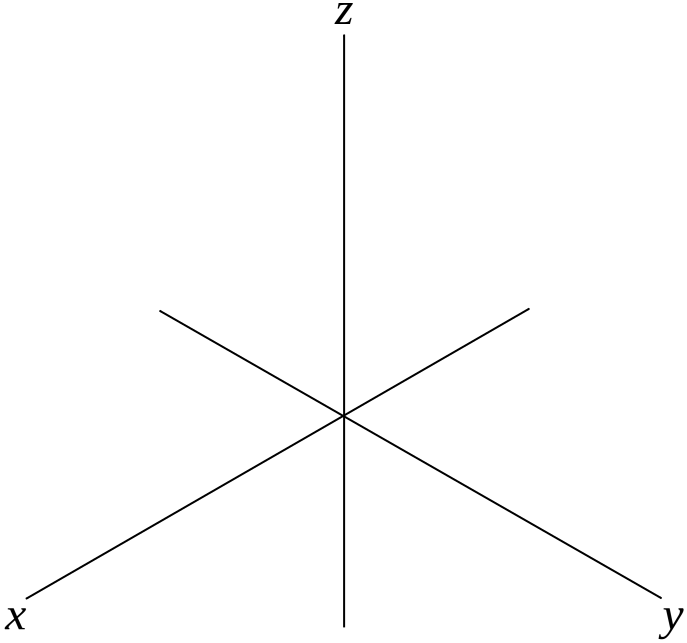
\includegraphics[scale=#1]{3DAxes}\end{center}}
\newcommand{\axespt}[1]{\begin{center}\includegraphics[scale=#1]{3DAxesWithPoint}\end{center}}
\newcommand{\pic}[2]{\begin{center}\includegraphics[scale=#1]{#2}\end{center}}
\newcommand{\comps}[1]{\langle #1_1,#1_2,#1_3\rangle}
\newcommand{\compslong}[3]{\langle #1, #2, #3\rangle}

\begin{document}
	\begin{flushright}
		{\large \textbf{Homework 2}}\hfill Name: \line(1,0){200}\\
		{\mbox{\hspace{1.75mm}}\small(front and back)}\hfill{\small (please print neatly!)}\mbox{\hspace{0.7in}}
	\end{flushright}
	\vspace{-1.5mm}
	\begin{adjustwidth}{0.5in}{0.5in}
		\begin{tcolorbox}[
			arc=0pt, colback=white, colframe=black, boxrule=0.5pt, before upper={\parindent15pt \parskip=3mm}]
			
			{\noindent\textbf{Directions:} Answer each of the following \textbf{\ul{six} (6)} questions, making sure to read the instructions for \ul{each question} as you proceed. \par
			
			\textbf{Make sure that your submission meets the criteria of the \ul{Homework Policy} on the \texttt{Homework} tab of the course webpage!}
				
			\hfill\textbf{Due date:} Friday, July 7}
		\end{tcolorbox}
	\end{adjustwidth}
		
	\begin{enumerate}
		\item Consider the second-order linear IVP
		\[(2x^2-7x+6)y''+\left(\frac{1}{2^x-1}\right)y'-\left(\frac{3\ln{x}}{\ln(\ln{x}))}\right)y=\frac{9\sqrt{x+1}}{\left(\ln{2x}\right)\left(\ln{x/3}\right)},\quad y(x_0)=y_0,\quad y'(x_0)=y'_0.\]
		For each of the following values $x_0$, state the largest interval on which the corresponding IVP has a unique solution \ul{or} state that no solution exists.
		\begin{adjustwidth}{0.75in}{-1.75in}
			\begin{multicols}{2}
				\begin{enumerate}[itemsep=0.75in]
					\item $x_0=2$
					\item $x_0=\frac{3+e}{2}$
					\item $x_0=\frac{-2.1}{4}$
					\item $x_0=e$
					\item $x_0=\frac{1}{2}$
					\item $x_0=\pi$
					\item $x_0=-1$
					\item $x_0=\frac{3}{2}$
					\item $x_0=\frac{3.1}{2}$
					\item $x_0=0$
					\item $x_0=\frac{9e}{10}$
					\item $x_0=5$
				\end{enumerate}
			\end{multicols}
		\end{adjustwidth}
		
		\newpage
		
		\item Find the Wronskian of the two solutions $y_1$ and $y_2$ of each of the following second-order linear ODEs. \textul{Do not attempt to solve the ODEs!}
		\begin{enumerate}[itemsep=1in]
			\item $y''-\frac{2}{x}y'+3xy=0$
			\item $e^xy''-\left(e^{2x}\sin{x}\right)y'-e^xy=0$
			\item $x^2y''+xy'+(x^2-\alpha^2)y=0$ where $\alpha=\const$
		\end{enumerate}
			
		\item A second-order linear homogeneous ODE $P(x)y''+Q(x)y'+R(x)y=0$ is said to be \textit{(second-order) exact} if it can be written in the form
		\begin{equation}
			\label{eq:1}[P(x)y']'+[f(x)y]'=0
		\end{equation}
		for some function $f(x)$. A well-known result in the theory of second-order ODEs is that $P(x)y''+Q(x)y'+R(x)y=0$ is (second-order) exact if and only if $P''(x)-Q'(x)+R(x)=0$.
		\begin{enumerate}[itemsep=0.5in]
			\item Show that $xy''-(\cos{x})y'+(\sin{x})y=0$ is (second-order) exact.
			\item Rewrite $xy''-(\cos{x})y'+(\sin{x})y=0$ in the form \eqref{eq:1}. \textbf{You don't know what $f(x)$ is yet!}
			\item Find $f(x)$ by expanding the left-hand side (LHS) of part (b) and comparing it term-by-term with the ODE $xy''-(\cos{x})y'+(\sin{x})y=0$.
			\item Reduce $xy''-(\cos{x})y'+(\sin{x})y=0$ to a \ul{first-order linear ODE} by integrating both sides of the result from (b) with respect to $x$. \textbf{Don't forget to plug in $f(x)$ from (c)!}
			\item The result from part (d) is a first-order linear ODE. Use it to solve for $y$ by
			\begin{itemize}[label=$\circ$]
				\item finding and multiplying both sides by its integrating factor (see \S2.1 for a refresher); and
				\item finding its general solution (ditto \S2.1).
			\end{itemize}
		\end{enumerate}
		
		\newpage
		
		\item For each of the following non-homogeneous ODEs, find the undetermined coefficients $A$, $B$, $C$, \textellipsis which make the indicated ``guess'' function $Y(x)$ a particular solution.
		\begin{enumerate}[itemsep=1.125in]
			\item $y''-2y'-2y=2x+4x^3$;\par\ul{Guess:} $Y(x)=Ax^3+Bx^2+Cx+D$
			\item $y''+2y'-3y=4\sin{2x}$;\par\ul{Guess:} $Y(x)=A\cos{2x}+B\sin{2x}$
			\item $y''+9y=6$;\par\ul{Guess:} $Y(x)=A$
			\item $y''+9y=x^2e^{3x}$;\par\ul{Guess:} $Y(x)=(Ax^2+Bx+C)e^{3x}$
		\end{enumerate}
		
		\vspace{0.5in}
		
		\item Using parts (c) and (d) above, find the general solution of the ODE $y''+9y=x^2e^{3x}+6$.\par\vspace{1.5mm}\hint{If the right-hand side (RHS) of a non-homogeneous ODE has the form $f(x)+g(x)$, you can 
		\begin{itemize}[label=$\circ$,itemsep=0mm]\vspace{-1.5mm}
			\item split up the RHS;
			\item use \ul{two} guesses---one called $Y_1(x)$ (corresponding to RHS=$f(x)$) and the other $Y_2(x)$ (for RHS=$g(x)$); 
			\item find the undetermined coefficients for each $Y_1$ and $Y_2$; and
			\item form the sum $Y_3=Y_1+Y_2$.
		\end{itemize}
		$Y_3$ (with the ``undetermined coefficients'' determined and plugged-in) will be the solution you seek!}
		
		\newpage
		
		\item Sometimes, the method of undetermined coefficients will lead you to guess a particular solution $Y(x)$ to the non-homogeneous ODE $ay''+by'+cy=g(x)$ which is \textit{also} a solution to the corresponding homogeneous ODE $ay''+by'+cy=0$. When this is true, we need a way to come up with a new guess.
		\begin{enumerate}[itemsep=0.7in]
			\item Show that $y_1=e^{-x}$ and $y_2=e^{4x}$ form a fundamental system of solutions for the homogeneous ODE $y''-3y'-4y=0$.
			\item Write down a reasonable guess $Y(x)$ (with undetermined coefficients) for a particular solution of the non-homogeneous ODE $y''-3y'-4y=2e^{-x}$. \hint{The answer is $Y(x)=Ae^{-x}$; now explain why.}
			\item Using your $Y$ from part (b), show that no combination of $A$, $B$, $C$, \textellipsis yields a valid particular solution having the form you guessed.
		\end{enumerate}
		\vspace{0.7in}
		\noindent When you run into a situation like the above, a good \ul{new} guess is \ul{$x$ times the thing you guessed before}.
		\begin{enumerate}[resume,topsep=1.5mm]
			\item Using the guess $Y(x)=Axe^{-x}$, find the coefficient $A$ which makes $Y$ a particular solution of the ODE $y''-3y'-4y=2e^{-x}$.
		\end{enumerate}
		\vspace{0.7in}
		\noindent Sometimes, both your first guess \textit{and} $x$ times your first guess will be elements of a fundamental system of solutions for the corresponding homogeneous ODE. This means you'll need \textit{another} new guess, and the next obvious choice is \ul{$x^2$ times the thing you guessed first}.
		\begin{enumerate}[resume,topsep=1.5mm,itemsep=0.7in]
			\item Show that $y_1=e^{-x}$ and $y_2=xe^{-x}$ form a fundamental system of solutions for the homogeneous ODE $y''+2y'+y=0$.
			\item Write down \textbf{two} reasonable guesses $Y_1(x)$ and $Y_2(x)$ (both with undetermined coefficients) for a particular solution of the non-homogeneous ODE $y''+2y'+y=2e^{-x}$. \hint{The answers are $Y_1(x)=Ae^{-x}$ and $Y_2(x)=Axe^{-x}$; once again, explain why.}
			\item Using the guess $Y(x)=Ax^2e^{-x}$, find the coefficient $A$ which makes $Y$ a particular solution of the ODE $y''+2y'+y=2e^{-x}$.
		\end{enumerate}
		
	\end{enumerate}
\end{document}